\documentclass[journal]{IEEEtran}
\usepackage{iftex}
\ifPDFTeX
\else
\usepackage{fontspec}
\setmainfont{texgyretermes-regular.otf}[
    BoldFont=texgyretermes-bold.otf,
    ItalicFont=texgyretermes-italic.otf,
    BoldItalicFont=texgyretermes-bolditalic.otf]
\setmonofont{lmmono10-regular.otf}
\fi
\usepackage{amsmath,amsfonts}
\usepackage{array}
\usepackage[caption=false,font=normalsize,labelfont=sf,textfont=sf]{subfig}
\usepackage{textcomp}
\usepackage{stfloats}
\usepackage{url}
\usepackage{verbatim}
\usepackage{graphicx}
\usepackage{cite}
\usepackage{tabularx}
\usepackage{booktabs} % For better looking tables

\hyphenation{op-tical net-works semi-conduc-tor IEEE-Xplore}

% NOTE: Mini Project report template for the undergraduate CS4486 AI course.
% The Mini Project is a Kaggle competition reproduction & improvement task.

% =========================================================================
% HOW TO USE THIS DRAFT
% - Text marked [TODO: ...] must be filled in before submission.
% - LaTeX comments starting with "% TODO(user):" carry notes for the team
%   and are NOT visible in the compiled PDF.
% =========================================================================

\begin{document}

% --------------------------------------------------------------------------
% TITLE & AUTHOR
% --------------------------------------------------------------------------
\title{CS4486 AI Course -- Mini Project Final Report:\\Mechanisms of Action Prediction}

% Confirm the registered group and fill actual Student IDs.
\author{\textbf{Group 11}\\[0.6em]
    Zifeng Xu (Group Leader) + 72400440 \\[0pt]
    Cheng Zong + 72400174 \\[0pt]
    Zibin Feng + 72400739
}
\markboth{CS4486 AI Course - Mini Project Final Report}%
{Group 11: Mechanisms of Action Prediction}
\maketitle

\begin{abstract}
Predicting a drug's mechanisms of action from cellular measurements requires learning rare, correlated labels while accounting for repeated experiments on the same compound. We study whether a drug-response prototype library improves a neural ensemble on the Kaggle Mechanisms of Action competition. The system combines two gated CNN configurations, a dual-head MLP, and similarity-weighted votes from training-drug prototypes. Evaluation uses fixed five-fold assignments, training-fold preprocessing, and cross-fitted fusion. The final treated-row out-of-fold log loss is 0.01672507, compared with 0.02287174 for a frequency baseline. Removing the library and refitting fusion increases loss by 0.00006490, the largest increase among the four source-removal comparisons. Kaggle submission 57940904 scores Public 0.01814 and Private 0.01590. The Private score improves on the group's reference threshold, while the Public score remains slightly higher. Validation limitations include nine drug groups spanning folds and epoch selection on held-out folds.\\
Kaggle code --- \url{https://www.kaggle.com/code/xiaozhanfen/moa-response-library}. Complete project repository --- [TODO: Add the URL after the repository is created].
\end{abstract}

\begin{IEEEkeywords}
Mechanisms of Action, Multi-label Classification, Drug-response Prototypes, Neural Ensembles, Cross-validation.
\end{IEEEkeywords}

\section{Task Description \& Metric}
\label{sec:task}

\subsection{Prediction Task}
Our project addresses Topic~2, \emph{Mechanism of Action Prediction with High-Dimensional Biological Data}, in the course's Intermediate tier. The Kaggle competition~\cite{ref_kaggle} provides gene-expression and cell-viability measurements after drug treatment. Predicting mechanisms of action (MoAs) from these cellular responses can help prioritize hypotheses for subsequent experiments. The competition is available at \url{https://www.kaggle.com/competitions/lish-moa}.

Each row is an experiment under a particular treatment time and dose. Inputs contain 772 gene readouts, 100 cell-viability readouts, and treatment metadata. The output is a marginal probability for each of 206 scored MoA labels. A compound can have several MoA annotations, making this a multi-label task. Direct neural heads use independent sigmoid transformations, and the model can assign substantial probability to several labels in one row. Training data also provide 402 auxiliary annotations and drug identifiers linking repeated measurements of a compound.

\subsection{Evaluation Metric}
The competition averages binary logarithmic loss over $N$ rows and 206 targets. Defining each entry's contribution as
\begin{equation}
\ell_{ij}=-y_{ij}\ln p_{ij}-(1-y_{ij})\ln(1-p_{ij}),
\end{equation}
the score is
\begin{equation}
L=\frac{1}{206N}\sum_{i=1}^{N}\sum_{j=1}^{206}\ell_{ij}.
\label{eq:logloss}
\end{equation}
Probabilities are clipped to $[10^{-15},1-10^{-15}]$ before evaluation. Lower loss is better. Predicting $p=0.001$ for a positive label incurs about 6.91 loss for that entry. Confident false positives also incur large penalties. These properties make probability quality central to both training and model selection.

\section{Data Analysis \& Challenges}
\label{sec:data}

\subsection{Dataset and Label Distribution}
Table~\ref{tab:data} summarizes the supplied data. An audit of the training and public test feature CSVs found zero missing cells and finite values in all 872 numeric columns. The drug mapping has 3,289 distinct identifiers including the control identifier, with 3,288 drugs among treated rows. Drug identifiers and auxiliary annotations are available in training.

\begin{table}[!t]
\caption{Data used in the project. Numeric inputs comprise 772 gene and 100 cell-viability measurements per row.}
\label{tab:data}
\centering
\begin{tabularx}{\columnwidth}{Xr}
\toprule
\textbf{Property} & \textbf{Count}\\
\midrule
Training rows & 23,814\\
Treated / control training rows & 21,948 / 1,866\\
Public test rows / controls & 3,982 / 358\\
Scored / auxiliary labels & 206 / 402\\
Drugs among treated training rows & 3,288\\
Distinct scored-label combinations & 328\\
Distinct joint annotation combinations & 696\\
\bottomrule
\end{tabularx}
\end{table}

Only 0.373\% of the $21{,}948\times206$ treated training label entries are positive. Per-label positive counts range from 1 to 832, with median 38.5. As Fig.~\ref{fig:label-frequency} shows, 53 labels have fewer than 20 positive examples. This distribution makes marginal frequencies a meaningful baseline and motivates parameter sharing and regularization.

\begin{figure}[!t]
\centering
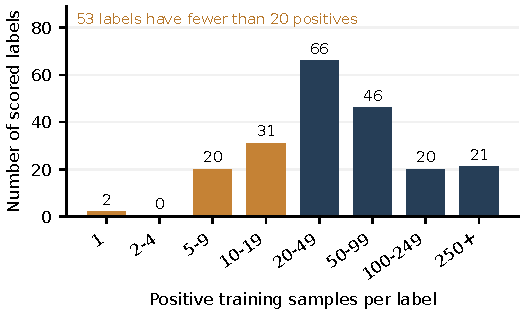
\includegraphics[width=\columnwidth]{figures/label_frequency.pdf}
\caption{Label support in treated training data. Each bar counts the scored labels whose positive sample counts fall in the indicated interval.}
\label{fig:label-frequency}
\end{figure}

Treatment duration is 24, 48, or 72 hours, with 7,166, 7,602, and 7,180 treated training rows, respectively. Doses D1 and D2 contain 11,196 and 10,752 rows. Controls are identified by \texttt{cp\_type=ctl\_vehicle} and have zero scored annotations.

\subsection{Consequences for Modeling}
The data suggest three modeling priorities. First, rare positives need shared representations and careful probability estimation. The 696 observed joint annotation patterns offer a way to share information across scored and auxiliary labels. Second, repeated measurements of one drug provide multiple observations of a common scored annotation, motivating response prototypes formed by averaging replicates. Third, those same replicates require explicit validation grouping. Samples from a drug observed during training can present an easier prediction problem than samples from an entirely unseen compound. These considerations determine the evaluation protocol and the components tested below.

\section{Validation Strategy}
\label{sec:validation}

\subsection{Fixed Drug-aware Folds}
The project uses the supplied frozen assignments in \path{data/folds.csv}, with split seed 42. All methods share these five folds, containing 4,389--4,390 treated validation rows each. Drugs with at most 18 treated records stay within one fold. Nine higher-frequency drugs can span folds, so some validation samples have same-drug replicates in training. This protocol supports consistent development comparisons, while its grouping limitation affects interpretation of unseen-drug performance.

For each neural configuration, five random seeds (0--4) are trained per fold. Each row's OOF probability averages the five models for its held-out fold. Across three configurations, CV trains $3\times5\times5=75$ networks. The deployment stage subsequently retrains eight seeds per configuration on all treated rows, giving 24 networks.

\subsection{Preprocessing, Fusion and Score Denominators}
Quantile transforms, PCA, factor analysis, auxiliary-label selection, the annotation-pattern vocabulary, and the response library are fitted using the current training fold. Validation rows receive the saved transformations. Control rows are excluded from model fitting, and their final probabilities are set to zero using the provided control indicator.

For fusion evaluation on fold $f$, blending parameters are fitted on OOF predictions and labels from the other four folds. A separate deployment fit uses all OOF rows. Each ablated source subset receives its own fusion fit under the same protocol.

Unless explicitly identified as full-row, local results report Eq.~\eqref{eq:logloss} on the 21,948 treated rows. Kaggle scores all test rows, including controls. Our full-row local score adds zeroed control predictions to the denominator. All validation losses use original binary labels, even when training applies label smoothing.

\subsection{Sources of Development Bias}
The best network epoch is selected using its held-out fold. Furthermore, the OOF predictions used to fit fusion on other folds come from base models whose training sets can include rows from fold $f$. Cross-fitting excludes fold $f$ from direct fusion fitting, while these underlying dependencies remain. We therefore interpret OOF results as development estimates and also report the official Kaggle scores. A fully nested evaluation would select epochs, fit preprocessing and train the fusion pipeline within each outer training split.

\section{Baseline Model}
\label{sec:baseline}

For scored label $j$, the baseline predicts the training-fold positive frequency
\begin{equation}
\widehat p_j=\frac{1}{|T|}\sum_{i\in T}y_{ij}
\end{equation}
for every treated validation row, with metric clipping applied at evaluation. Here $T$ contains treated training rows from four folds. This is the empirical log-loss optimum among constant probabilities for that label. Control predictions are set to zero.

The baseline OOF loss is \textbf{0.02287174} on treated rows and 0.02107958 on all rows. It requires no feature fitting, optimization schedule or neural weights and is implemented in \texttt{baseline.py}. Subsequent comparisons measure whether using cellular measurements and response structure improves on these label priors under the same frozen assignments.

\section{Model Improvements}
\label{sec:improvements}

\subsection{Design Rationale and Method Sources}
Our central question is whether training-drug response prototypes add predictive information to a diverse neural ensemble. The neural component learns discriminative feature representations and label structure. The library summarizes repeated responses and contributes probability votes according to response similarity. Figure~\ref{fig:model-overview} shows how their outputs enter the final prediction.

All networks are trained from random initialization. Sample normalization, projection before convolution, and auxiliary-label warm-up draw on the public second-place solution~\cite{ref_moa2nd}. The MLP feature design draws on the first-place write-up~\cite{ref_moa1st}. Gating, auxiliary selection, the pattern head, the response library and the fusion analysis are project-specific implementations. AI participation is detailed in Section~\ref{sec:ai}.

\begin{figure*}[!t]
\centering
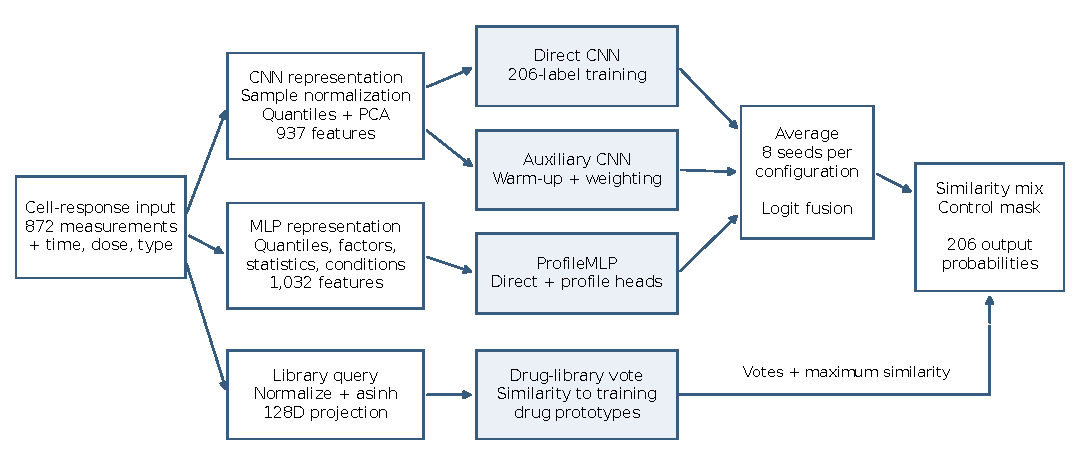
\includegraphics[width=0.98\textwidth]{figures/model_overview.pdf}
\caption{Deployment prediction flow. Each neural configuration averages eight seeds. Library queries use a projection and drug prototypes fitted on training data. The final blend uses the library's votes and maximum response similarity, then applies the control indicator. CV uses five seeds per configuration and training-fold fitted transformations and prototypes.}
\label{fig:model-overview}
\end{figure*}

\subsection{Two Neural Representations and Three Configurations}
\textbf{CNN representation.} Gene and cell blocks are centered separately within each sample at the midpoint of their 25th and 75th percentiles. The centered cell block is divided by four plus the 75th percentile of its absolute values. Training-fold quantile transforms map each column toward a normal distribution. The original 872 transformed measurements are concatenated with 50 gene and 15 cell PCA coordinates, scaled by their training standard deviations, producing 937 inputs.

\textbf{Direct CNN.} A fully connected projection maps these inputs to 4,096 values, reshaped into 256 channels and 16 learned positions. Thus the convolutions operate on a learned representation of the measurements. Two convolutional stages and a sigmoid gate produce features multiplied by a factor in $[0,2]$, followed by pooling and a 206-logit head. The deployment network has 5,690,912 trainable parameters. Appendix~\ref{app:implementation} provides the stage dimensions.

\textbf{Auxiliary CNN.} This configuration uses the same architecture. Within each training fold, auxiliary labels are ranked by their maximum absolute Pearson correlation with any scored label. A temporary head trains for one epoch on the top 33 labels. The original randomly initialized scored head is restored, and the model is fine-tuned on the scored task. Positive terms receive frequency weight
\begin{equation}
w_j=\frac{\ln(100+n_{\min})}{\ln(100+n_j)},
\end{equation}
where $n_j$ is the training-fold positive count for label $j$ and $n_{\min}$ is the minimum count. This gives lower weight to frequent positive labels. Warm-up and weighting were introduced together in the recorded comparison.

\textbf{ProfileMLP.} The second representation contains 872 quantile-transformed measurements, 90 gene and 50 cell factor-analysis coordinates, 15 block statistics, and five time/dose indicators. A second quantile transform acts on the concatenated 1,032 inputs. Statistics comprise sum, mean, standard deviation, kurtosis and skewness for gene, cell and combined blocks, computed after the first quantile transform.

The MLP uses two hidden layers of width 2,048, LeakyReLU, BatchNorm, dropout and weight normalization on its first and output layers. One output head predicts scored labels directly. The other predicts observed joint patterns of the 206 scored and 402 auxiliary annotations, using a vocabulary constructed within the training fold. If $C$ maps patterns to their scored labels and $z$ is the pattern-head output, its scored marginal probabilities are
\begin{equation}
p_{\mathrm{pattern}}=\operatorname{softmax}(z)C.
\end{equation}
These probabilities are averaged equally with the direct head's sigmoid outputs. Training minimizes mean scored-label BCE plus pattern cross-entropy divided by 206. The pattern head incorporates observed co-occurrence structure, while the direct head can assign probability outside those observed patterns. The all-data deployment MLP has 8,173,340 trainable parameters, with its output width depending on the annotation vocabulary.

\subsection{Drug-response Prototype Library}
The library uses drug identifiers only while fitting training prototypes. Measurements are sample-normalized, transformed with $\operatorname{asinh}$, and standardized using training-column statistics. Averaging by drug gives a response prototype, while replicate residuals estimate within-drug variation. A regularized generalized eigenproblem contrasts between-drug and within-drug variation to obtain 128 projection directions.

A query is projected and normalized, then compared with normalized prototypes by cosine similarity. For prototype $d$, with similarity $s_d$ and $n_d$ training replicates, the voting weight and predicted label vector are
\begin{equation}
\alpha_d=\frac{\exp(24s_d+\ln n_d)}{\sum_k\exp(24s_k+\ln n_k)},
\quad p_{\mathrm{lib}}=\sum_d\alpha_d y_d.
\end{equation}
The all-data library contains 3,288 prototypes. Each CV library uses the drugs present in its training fold. Test drug identifiers are unnecessary for this computation because queries use measured responses.

\subsection{Fusion and Library Weighting}
Within each configuration, seed probabilities are averaged before conversion to logits. For configuration probabilities $p_k$, neural fusion uses
\begin{equation}
p_{\mathrm{NN}}=\sigma\!\left(b+\sum_{k=1}^{3}a_k\operatorname{logit}(p_k)\right).
\label{eq:blend}
\end{equation}
Let $c$ be the maximum prototype similarity clipped to $[0,1]$. The library gate and final probability are
\begin{equation}
\begin{aligned}
g(c)&=g_{\mathrm{low}}(1-c)+g_{\mathrm{high}}c,\\
p_{\mathrm{final}}&=(1-g(c))p_{\mathrm{NN}}+g(c)p_{\mathrm{lib}}.
\end{aligned}
\label{eq:libmix}
\end{equation}
L-BFGS-B minimizes treated-row log loss over nonnegative neural coefficients bounded to $[0,3]$, an unconstrained intercept and two library endpoints bounded to $[0,0.6]$. This learns the blend and its calibration jointly. The all-OOF deployment fit gives $g_{\mathrm{low}}=0$ and $g_{\mathrm{high}}=0.250143$, so closer prototype matches receive greater library weight. Validation fits are specific to each held-out fold and source subset. Exact deployment coefficients are provided in Appendix~\ref{app:implementation}.

\subsection{Component Evaluation}
Table~\ref{tab:ablation} reports original branch probabilities under the common five-fold protocol. The auxiliary CNN improves slightly on the direct CNN after the joint warm-up and weighting change. The MLP has the highest standalone loss of the three branches.

\begin{table}[!t]
\caption{Standalone neural branch performance, before additional fusion calibration. Each branch averages five seeds per held-out fold.}
\label{tab:ablation}
\centering
\begin{tabularx}{\columnwidth}{Xr}
\toprule
\textbf{Configuration} & \textbf{Treated OOF loss}\\
\midrule
Direct CNN & 0.01701975\\
Auxiliary CNN & \textbf{0.01698392}\\
ProfileMLP & 0.01708700\\
\bottomrule
\end{tabularx}
\end{table}

For the ensemble analysis, we keep all base predictions fixed and refit fusion for each source subset. The complete system has the lowest development loss among 15 nonempty combinations (Appendix~\ref{app:combinations}). Figure~\ref{fig:source-removal} shows the effect of removing each source. Removing ProfileMLP costs more than removing either CNN, supporting its inclusion despite its weaker standalone result. Removing the library raises loss from 0.01672507 to 0.01678997, a difference of 0.00006490, or about 0.387\% of the neural-only loss. These contrasts include refitting fusion for the remaining sources.

\begin{figure}[!t]
\centering
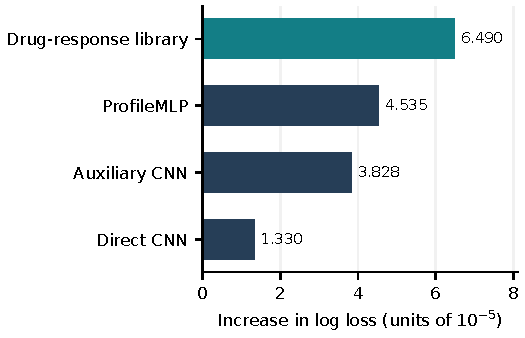
\includegraphics[width=\columnwidth]{figures/source_removal.pdf}
\caption{Increase in treated-row OOF loss after removing one prediction source and refitting fusion. The full-system reference is 0.01672507. Bars show conditional source-removal effects under the shared development protocol.}
\label{fig:source-removal}
\end{figure}

\section{Final Results}
\label{sec:results}

\subsection{Development Results and Earlier Reference}
Table~\ref{tab:results} collects the principal results. The complete system reduces treated-row loss by 26.9\% relative to the frequency baseline. Including zeroed controls gives full-row OOF loss 0.01541454. The CV and deployment rows describe their respective fitted systems and seed counts.

\begin{table*}[!t]
\caption{Principal results. Local OOF scores use treated rows. The deployment row contains the official scores of submission 57940904, Version~1.}
\label{tab:results}
\centering
\begin{tabularx}{0.95\textwidth}{Xrrr}
\toprule
\textbf{System} & \textbf{Treated OOF loss} & \textbf{Public LB} & \textbf{Private LB}\\
\midrule
Frequency baseline & 0.02287174 & --- & ---\\
Auxiliary CNN, five seeds per fold & 0.01698392 & --- & ---\\
Three-configuration neural fusion & 0.01678997 & --- & ---\\
Full system, CV configuration & \textbf{0.01672507} & --- & ---\\
Full system, 24-network deployment & --- & \textbf{0.01814} & \textbf{0.01590}\\
\bottomrule
\end{tabularx}
\end{table*}

We also compare with an earlier internal system, Course5, whose treated-row OOF loss is 0.01706366. The final system improves on this earlier reference in all five folds (Fig.~\ref{fig:fold-comparison}). A paired drug-cluster bootstrap resamples drugs with replacement for 1,200 draws, using seed 4486, and computes the row-weighted loss difference in each draw. The resulting 95\% interval is $[-0.000414,-0.000266]$. This interval describes the complete-system comparison with Course5. The library's conditional contribution is quantified by the separate source-removal contrast.

\begin{figure}[!t]
\centering
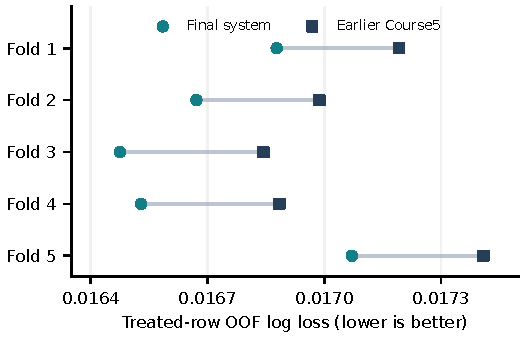
\includegraphics[width=\columnwidth]{figures/fold_comparison.pdf}
\caption{Paired fold scores for the earlier Course5 system and the final system, using the same treated validation rows. The final system improves in every fold. The bootstrap interval in the text uses drugs as clusters.}
\label{fig:fold-comparison}
\end{figure}

\subsection{Kaggle Scores and the Course Target}
The final Kaggle scores are Public 0.01814 and Private 0.01590. The earlier Course5 submission, 57937726, scored Public 0.01866 and Private 0.01629. Both official scores improve in the same direction as local CV, while Public and Private evaluate different test subsets.

The reference thresholds used in the group's presentation are Public 0.01805 and Private 0.01602. The final Private score is lower by 0.00012, while the Public score is higher by 0.00009. The course's Case~A criterion refers to leaderboard placement. [TODO: Verify the original source, date and ranking associated with these reference scores, and the applicable interpretation of the Top-5 requirement.]

\section{AI Tool Usage Statement}
\label{sec:ai}

OpenAI Codex participated in modeling discussion, technical explanation, code development and debugging, experimental analysis, and preparation and revision of project materials, including this report and its visualizations. The project records acknowledge AI participation in model development and implementation. Public method sources are cited in Section~\ref{sec:improvements}.

The group reports the following division of responsibility. Zibin Feng handled data analysis, the frequency baseline and report writing. Cheng Zong handled the main model modules and fusion design. Zifeng Xu handled training runs, experiments, Kaggle submission, ablations and result analysis. These responsibilities describe the work areas within the AI-assisted project.

[TODO: Each member should verify the disclosed AI tools and uses, identify the parts independently completed, and record how code and experimental results were checked. Add any additional AI tools actually used.]

\section{Discussion \& Reflection}
\label{sec:discussion}

\subsection{What the Comparisons Establish}
The source-removal results support retaining both neural architectures and the response library. ProfileMLP contributes in combination despite having a weaker standalone score. Its annotation-pattern supervision provides a plausible explanation for complementary errors, although the experiments combine that head with its wider feature pipeline and architecture. The replicate-based library is motivated by averaging response noise and comparing queries with training-drug profiles. Its measured gain is conditional on the remaining sources and the refitted fusion.

Auxiliary warm-up and frequency weighting improve the CNN together. Their individual contributions require separate controls. Similarly, improvements from a calibrated ensemble include the effect of calibration and combining predictions. The recorded studies support the complete configurations evaluated here.

\subsection{Failure Cases}
The improvement over Course5 is uneven across labels. Of 206 labels, 150 improve in OOF loss, while \texttt{hcv\_inhibitor} worsens. Table~\ref{tab:failures} shows two selected positive entries that receive very low probabilities. Their entry losses are approximately 7.26 and 7.63. These cases demonstrate the cost of missed positives under log loss, while an aggregate analysis would be needed to quantify how broadly this failure pattern occurs.

\begin{table}[!t]
\caption{Selected missed positives from final OOF predictions. Both ground-truth labels equal one. Full sample identifiers are recorded with the experiment artifacts.}
\label{tab:failures}
\centering
\begin{tabularx}{\columnwidth}{Xr}
\toprule
\textbf{Positive target and sample} & \textbf{Predicted probability}\\
\midrule
HCV inhibitor, \texttt{id\_3ab03dc25} & 0.0007008\\
Nitric oxide production inhibitor, \texttt{id\_344ef5019} & 0.0004833\\
\bottomrule
\end{tabularx}
\end{table}

\subsection{Limits and Next Experiments}
Nine drugs can occur across training and validation folds. Epoch selection uses validation performance, and the fusion protocol retains dependencies between base-model training sets. Repeated development comparisons also reuse the fixed OOF data. A stronger evaluation would use drug-disjoint outer folds and make epoch and fusion decisions entirely within each outer training split.

Further experiments could isolate warm-up from frequency weighting, separate the MLP pattern head from its feature representation, and evaluate rare-label calibration. Each would address a specific uncertainty in the present interpretation. The Public score remains above the group's reference, and additional changes would need experimental validation before assigning them a likely benefit.

\section{Reproducibility}
\label{sec:reproducibility}

\subsection{Training and Deployment Settings}
CV uses split seed 42 and network seeds 0--4. Deployment uses seeds 0--7 for each of three configurations. All main tasks use Adam, weight decay $10^{-5}$, label smoothing 0.001 and a 25-epoch OneCycle schedule. Maximum learning rate is 0.01, with \texttt{pct\_start}=0.1 and \texttt{div\_factor}=1000. The schedule sets its initial learning rate from the maximum and division factor. CNN and MLP batch sizes are 128 and 256, respectively. Main dropout is 0.2 for CNNs and 0.25 for ProfileMLP.

The auxiliary warm-up lasts one epoch, with weight decay $10^{-4}$, before a fresh main-task optimizer is created. Deployment stopping epochs are the median CV checkpoint epochs, 18 for direct CNN, 7 for ProfileMLP and 22 for auxiliary CNN. Their learning-rate schedules retain a total length of 25 epochs. The scored bundle uses per-row INT8 weight storage and totals 113.96~MB. Quantization changed the audited fold-0 loss by approximately $1.6\times10^{-7}$. CPU inference regenerates predictions from the raw measurements.

The recorded environment is Python 3.11.17, PyTorch 2.11.0+cu128, CUDA 12.8 and an RTX~5080 with 16~GB VRAM, using BF16 during training. [TODO: Confirm the original training operating system and version.] The dependency file pins NumPy, pandas, SciPy and scikit-learn, specifies a range for \texttt{nbformat}, and requires a separately installed PyTorch build. Retraining can vary across hardware and library builds.

\subsection{Code, Data and Commands}
The scored Kaggle notebook is available at \url{https://www.kaggle.com/code/xiaozhanfen/moa-response-library}. Its associated weights and inference modules are identified by \url{https://www.kaggle.com/datasets/xiaozhanfen/moa-response-library-weights}. Complete training code, frozen folds, analysis scripts and report figures will be linked through the project repository. [TODO: Add the repository URL after creation and verify reviewer access to the Kaggle notebook and dataset.]

Place the six official competition CSVs under \path{data/raw/}, retain the supplied \path{data/folds.csv}, and install the appropriate PyTorch build. The comparative study also uses the supplied predictions and statistics under \path{evidence/baseline_course5/}. From the project root, the main commands are
\begin{verbatim}
python -m pip install -r requirements.txt
python predict.py
python verify_project.py
python baseline.py
python reproduce.py all
\end{verbatim}
Retraining writes its CV, study, audit, full-data and packaging artifacts under \path{reproduction/}. The scored Version~1 bundle is stored under \path{response_release/}. Inference alone requires the raw test features, submission template and saved weights.

The script \path{preparation/evaluate_report_combinations.py} reconstructs the 15-source-combination results from aligned base OOF predictions and saves \path{evidence/report_combinations.json}. It refits each neural subset's fusion on four folds and applies it to the fifth. The library-only result uses saved similarity votes. This analysis requires the saved OOF arrays or their regeneration by the CV stage. The script \path{preparation/generate_report_figures.py}, using Matplotlib, regenerates all four figures from the official data and recorded results.

% --------------------------------------------------------------------------
% SECTION 10: STUDENT BIO & REFLECTION
% --------------------------------------------------------------------------
\section{Student Bio and Self-Reflection}
\label{sec:bio}

% English spellings are transliterations. Confirm preferred spellings before submission.
% Speaker mapping from the presentation and the group leader's account:
% A = Feng Zibin, B = Zong Cheng, C = Xu Zifeng.
[TODO: Each member should review the drafted reflection below and amend it to match their own experience and preferred English name.]

\subsection{Zibin Feng, Student ID 72400739}
\textbf{Biography.} Zibin Feng is a CS4486 project member whose technical focus in this project was data analysis, baseline construction and technical reporting.

\textbf{Self-reflection.} My main takeaway is that a baseline needs to reflect the data distribution and the evaluation protocol. With sparse labels, marginal frequencies already produce a low log loss. The learned system's improvement becomes meaningful when both methods use the same rows and folds. Preparing the report also highlighted the need to explain whether a result measures a standalone model, calibrated fusion or a component-removal comparison.

\textbf{Contribution.} I handled dataset analysis, the frequency baseline and report writing, corresponding to the task, data, validation and baseline material presented by Speaker~A.

\subsection{Cheng Zong, Student ID 72400174}
\textbf{Biography.} Cheng Zong is a CS4486 project member whose technical focus was the main model modules and prediction fusion.

\textbf{Self-reflection.} The main lesson from the model and fusion work is that the strongest standalone branch need not provide the largest contribution to an ensemble. ProfileMLP has a weaker individual score but its removal increases the final loss more than removing either CNN. This motivates evaluating each source within the complete system. I would next isolate the pattern head and feature pipeline, and test warm-up and positive weighting separately, to obtain more specific evidence about the design choices.

\textbf{Contribution.} I handled the design of the main model modules and fusion, corresponding to the feature pipelines, neural configurations and response-library fusion explained by Speaker~B.

\subsection{Zifeng Xu, Student ID 72400440}
\textbf{Biography.} Zifeng Xu is the group leader and focused on training, experiment execution, submission and result analysis for this project.

\textbf{Self-reflection.} Running the experiments and submission emphasized the importance of keeping folds, seeds, artifacts and score definitions traceable. The source-removal study quantified how much the library and each neural branch contributed after fusion was refitted. The failure analysis and nine drugs spanning folds also showed why a better development score needs careful interpretation. A future evaluation should choose epochs and fusion configurations within a fully held-out outer training split.

\textbf{Contribution.} I handled training runs, experiments, Kaggle submission, ablations and result analysis. This corresponds to the results, failure cases and reproducibility material presented by Speaker~C.

% --------------------------------------------------------------------------
% SECTION 11: RELATIVE CONTRIBUTION
% --------------------------------------------------------------------------
\section{Relative Contribution}
\label{sec:contribution}

Table~\ref{tab:contributions} gives a provisional estimate based on the declared division of work. [TODO: Each member must confirm or correct these estimates against actual productive hours before submission. Exclude unattended model-running time and update the totals after any correction.]

% TODO(user): Confirm the proposed hours with every member and recalculate totals.

\begin{table*}[!t]
\caption{Provisional Contribution Breakdown in Hours, Pending Member Confirmation}
\label{tab:contributions}
\centering
\renewcommand{\arraystretch}{1.3}
\begin{tabularx}{0.9\textwidth}{|l|X|X|X|X|X|c|}
\hline
\textbf{Team Member} & \textbf{Data \& Validation} & \textbf{Baseline} & \textbf{Model Changes} & \textbf{Experiments \& Tuning} & \textbf{Report \& Slides} & \textbf{Total} \\
\hline
Zibin Feng & 8 & 6 & 0 & 2 & 12 & \textbf{28} \\
\hline
Cheng Zong & 3 & 1 & 18 & 6 & 2 & \textbf{30} \\
\hline
Zifeng Xu & 4 & 0 & 4 & 20 & 4 & \textbf{32} \\
\hline
\textbf{Team Total} & \textbf{15} & \textbf{7} & \textbf{22} & \textbf{28} & \textbf{18} & \textbf{90} \\
\hline
\end{tabularx}
\end{table*}

\section*{Team Leader Attestation}
``I, Zifeng Xu, confirm that the contributions listed above accurately reflect the work completed by each team member.'' \\
\vspace{0.5cm}
Signed: \_\_\_\_\_\_\_\_\_\_\_\_\_\_\_\_\_\_\_\_\_\_\_\_

\appendices
\section{Prediction-Source Combinations}
\label{app:combinations}

Table~\ref{tab:all-combinations} contains the 15 nonempty combinations of the neural sources and the library. Each neural subset includes fold-specific fusion and calibration, including subsets with one branch. Table~\ref{tab:ablation} reports the original branch probabilities. The library-only row uses its original similarity votes. All scores use the same treated validation rows.

\begin{table}[!ht]
\caption{All prediction-source combinations. D denotes direct CNN, A denotes auxiliary CNN, and M denotes ProfileMLP.}
\label{tab:all-combinations}
\centering
\begin{tabularx}{\columnwidth}{Xrr}
\toprule
\textbf{Neural sources} & \textbf{Without library} & \textbf{With library} \\
\midrule
None & --- & 0.02021583 \\
D & 0.01694366 & 0.01683897 \\
A & 0.01693918 & 0.01681519 \\
M & 0.01704105 & 0.01691114 \\
D + A & 0.01685988 & 0.01677042 \\
D + M & 0.01683135 & 0.01676334 \\
A + M & 0.01681193 & 0.01673837 \\
D + A + M & 0.01678997 & \textbf{0.01672507} \\
\bottomrule
\end{tabularx}
\end{table}

\section{Architecture and Deployment Parameters}
\label{app:implementation}

The CNN input projection produces $B\times256\times16$ features. A kernel-5 convolution maps 256 channels to 384, followed by average pooling to eight positions. A kernel-3 convolution retains 384 channels. The gate uses kernel-3 and kernel-1 convolutions with a final sigmoid, and multiplies the main features by twice the gate value. Final max pooling gives $B\times384\times4$ features, flattened to 1,536 values and mapped to 206 logits. BatchNorm, nonlinearities and dropout are applied as specified in \texttt{models.py}.

For Eq.~\eqref{eq:blend}, the all-OOF deployment coefficients, in direct CNN / ProfileMLP / auxiliary CNN order, are $(0.279946,0.379818,0.450498)$, with intercept 0.465227. Equation~\eqref{eq:libmix} uses library endpoints $(0,0.250143)$. These parameters are jointly fitted for deployment. Each validation fold and source subset fits its own parameters.

% --------------------------------------------------------------------------
% REFERENCES
% --------------------------------------------------------------------------
\begin{thebibliography}{3}
\bibliographystyle{IEEEtran}

\bibitem{ref_kaggle}
Kaggle and Laboratory for Innovation Science at Harvard, ``Mechanisms of Action (MoA) Prediction,'' Kaggle competition. [Online]. Available: \url{https://www.kaggle.com/competitions/lish-moa}

\bibitem{ref_moa2nd}
B.~Guo, ``Kaggle-MoA 2nd Place Solution,'' GitHub repository. [Online]. Available: \url{https://github.com/baosenguo/Kaggle-MoA-2nd-Place-Solution}

\bibitem{ref_moa1st}
``1st place winning solution -- hungry for gold,'' Kaggle competition write-up for Mechanisms of Action (MoA) Prediction. [Online]. Available: \url{https://www.kaggle.com/competitions/lish-moa/writeups/hungry-for-gold-1st-place-winning-solution-hungry-}

\end{thebibliography}

\end{document}
